\documentclass[11pt]{article}
\usepackage[utf8]{inputenc}
\usepackage{amsmath,amssymb}
\usepackage{graphicx}
\usepackage{booktabs}
\usepackage{authblk}
\usepackage[margin=1in]{geometry}
\usepackage{xcolor}
\usepackage[numbers,square]{natbib}
\usepackage[colorlinks=true,allcolors=blue]{hyperref}
\usepackage{caption}
\captionsetup{font=small}

\title{\textbf{At-Grok Is Not Converged:\\ A Measurement-Validity Audit for Grokking Representation Metrics}}
\author[1]{Truong Xuan Khanh}
\author[1]{Luu Duc Trung}
\affil[1]{H\&K Research Studio / Clevix LLC, Hanoi, Vietnam}
\affil[ ]{\texttt{khanh@clevix.vn}}
\date{}

\begin{document}
\setlength{\emergencystretch}{2em}
\maketitle

\begin{abstract}
A growing body of grokking research reads representation structure from a snapshot taken at the
generalization transition and treats it as a property of the converged circuit. We show that this is
unsafe in a specific and consequential way. The value of a standard representation metric, embedding
effective rank, read at the transition can be a transient that long training drives down to a low-rank
floor, across two regularization protocols and three tasks. The at-grok value then does not describe the
converged solution, and reading it can reverse the dependence one set out to characterize. That grokking
involves compression is not itself new; it is documented under complexity, intrinsic-dimension,
topological, and construct-then-compress accounts. Both the metric and the norm-clamp intervention are
standard, and we borrow them deliberately, because a measurement-reliability result has to exercise the
field's own metric under a standard intervention. A new metric or protocol would confound ``the common
measurement is unreliable'' with ``a different metric behaves differently.'' The contribution is a
measurement discipline and the tooling that enforces it. We give a measurement-validity audit that
separates generalization onset ($T_{\mathrm{grok}}$) from representation compression
($T_{\mathrm{compress}}$), flags censoring, excludes boundary cells that did not fully generalize, and
declines an ordering verdict when the order statistic is undefined. Applying it to two modular tasks
($16$ budget cells in total), we find that generalization precedes rank compression by a large lag, of
order $2\times10^4$ steps and comparable to $T_{\mathrm{grok}}$ itself, well beyond the
accuracy-to-topology lag reported elsewhere. The separation is the part that is robust: on the enlarged
grid the norm budget strongly orders $T_{\mathrm{grok}}$ but not the compression time, so we report a
large separation of the two times rather than a single shared clock. A secondary observation, which we
hold to a higher bar, is that on the MLP the norm budget sets, almost deterministically, how far the
representation compresses, with the converged effective-rank floor decreasing monotonically with the
budget (Spearman $-1.0$ at both tasks). We treat this depth law as a hypothesis and put it through a
pre-registered generality test, which it fails: it is protocol-specific (under free weight decay the
floor orders oppositely) and does not replicate on a well-powered transformer clamp sweep trained to
convergence (Spearman $+0.1$ on the embedding against $-1.0$ on the MLP). We report this negative result
as the same standard applied to our own secondary claim: the depth law is specific to the modular MLP and
is not a general norm law. The audit ships with an adversarial test suite that checks the reason behind
each verdict; it caught a false-confidence regression during development and, on the enlarged grid,
corrected our own earlier reading of the ordering. The transformer sweep also shows the central claim to
be general: the at-grok transient recurs on the embedding and the unembedding, is metric-agnostic, and is
present at every weight and activation locus, and the large compression lag returns, so the measurement
hazard, unlike the depth law, does not depend on architecture. The transformer overstatement is smaller
($1.3$--$1.5\times$ against $3$--$5\times$ on the MLP), but this does not soften the hazard. The error is
qualitative, a transition-time reading mistaken for a converged one, rather than a matter of magnitude,
and on the MLP that same error turns a monotone budget-dependence into a flat one and erases which cells
compress at all.
\end{abstract}

\section{Introduction}
Grokking, delayed generalization long after a network fits its training set
\citep{power2022grokking}, is increasingly studied through the representation: the Fourier
structure of embeddings \citep{nanda2023progress}, effective rank or spectral-entropy complexity
\citep{demoss2024complexity}, intrinsic dimension, and persistent homology \citep{tang2026topological}.
A recurring move in this literature is to take a measurement at or near the grokking step, the moment
test accuracy rises, and read it as a property of the generalizing circuit.

This move has a failure mode that is easy to hit and hard to notice: the value of a representation
metric at the grokking step need not be its converged value, and reading it can reverse the dependence
one set out to characterize. On modular arithmetic we find a sharp instance. At grokking the embedding
effective rank is uniformly high and barely separates across budgets at the low-budget end. The
non-compressing boundary cell ($\rho=1.00$, which never compresses and stays at rank $\approx\!42$) and
its strongly-compressing neighbour ($\rho=1.05$, which converges to rank $\approx\!12$) read almost
identically at grok ($\approx\!46$ vs.\ $\approx\!48$). Stopping there, the natural reading is a high,
flat ``norm-controlled circuit complexity,'' which is exactly backwards: training each fully-generalizing
budget long past the transition drives its rank down to a low-rank floor, while the boundary cell stays
high.
The at-grok snapshot overstates the converged complexity by $\approx\!3$--$5\times$ and hides the one
distinction that matters (which cells compress at all). The at-grok measurement was a transient on the
way to a budget-ordered compressed endpoint; this is consistent with the rise-and-fall of complexity
reported by \citet{demoss2024complexity}, whose peak sits near the transition --- precisely where these
snapshots are read.

\paragraph{What is and is not new here.} That grokking involves compression is not our claim
to make: it is by now well documented. \citet{demoss2024complexity} track a Kolmogorov/MDL complexity
that rises during memorization and falls at generalization; \citet{tang2026topological} report that
local intrinsic dimension drops (compression onto a low-dimensional manifold) around grokking while
persistent homology reveals a loop that emerges only after that compression; and geometric analyses of
transformers describe ``construct-then-compress'' dynamics with an explicit post-grokking
refinement phase. Our concern is therefore not whether compression occurs but whether a representation metric measured
at the transition is safe to read as a converged-circuit measurement. On modular arithmetic the answer is
often no, and the consequence is a reusable audit that separates generalization onset from compression,
quantifies the lag between them as a function of the norm budget, handles censoring and boundary cells,
and refuses an ordering verdict it cannot support. We use a standard metric (effective rank) under a standard intervention (the norm clamp)
\emph{by design}: the question is whether the field's own measurement, applied as the field applies it,
is reliable, and substituting a new metric or protocol would confound that question with ``a different
quantity behaves differently.'' The contribution is therefore a measurement discipline and the tooling
that enforces it, plus the quantitative lag it reveals; it belongs to a small but established
measurement-reliability strand: \citet{miller2024sharpness} make the train/test curves themselves
noise-robust and assumption-checkable, and \citet{prakash2026antigrokking} ask which structural
diagnostics stay faithful into late training. It targets a general practice, reading
representation structure at the transition, rather than any single result, and it is not the rediscovery of
compression.

\paragraph{Contributions.} Our findings sit at two confidence tiers, kept distinct throughout. The central result is
architecture-general and well supported: the at-grok transient and the grok-to-compression lag, both
validated on a transformer trained to convergence. The secondary observation is deliberately narrower:
the MLP depth law, which our own pre-registered generality test falsifies. We say which is which at every
step, and the negative result on the secondary claim is reported as the same standard applied to
ourselves.
\begin{itemize}
\item \textbf{An at-grok-vs-converged audit.} We show, on modular addition and multiplication MLPs,
that embedding effective rank at grokking is a transient peak that collapses under long training; the
converged solution is low-rank at every fully-generalized norm budget (the one budget that only
partially generalizes is the boundary case that does not compress, and the audit gates it out). The
transient is not an artifact of the clamp intervention or of arithmetic: it recurs under a free
weight-decay protocol and on parity, with the at-grok rank exceeding the converged floor in every
generalizing cell across three tasks and both protocols.
\item \textbf{A compression-lag diagnostic.} We define $T_{\mathrm{grok}}$, $T_{\mathrm{compress}}$,
their lag, a censoring flag, and a boundary gate that excludes cells which did not fully generalize.
The audit reports a large separation of the two times for both tasks, with generalization preceding
compression by a lag of order $T_{\mathrm{grok}}$, while explicitly declining a single-clock claim:
on the enlarged budget grid the compression time is not ordered by the norm budget the way
$T_{\mathrm{grok}}$ is, so we do not claim the two move as one clock.
\item \textbf{What the norm budget controls (a secondary, self-falsified observation).} On the MLP,
across the grid the norm budget sets, almost
deterministically, the depth of compression rather than its timing: the converged effective-rank
floor decreases monotonically with the budget (Spearman $-1.0$ at both tasks), and a higher budget
already pre-compresses the rank read at grokking (Spearman $\approx\!-0.97$). This both sharpens the
``transient'' picture and explains why the compression time is weakly ordered, since a later-grokking,
high-budget cell starts compression from an already-lower rank. We are careful to scope this, and then to
break it ourselves: the depth law's \emph{direction} is specific to the norm-clamp protocol (a free
weight-decay sweep orders the floor oppositely; \S\ref{sec:limitations}), and a transformer clamp sweep
trained to convergence shows the floor does not order with the budget at all on a second architecture
(\S\ref{sec:transformer}), so we report it as an MLP-specific regularity rather than a protocol- or
architecture-independent law.
\item \textbf{A test suite that enforces honesty.} An adversarial synthetic suite checks that the audit
does not fabricate compression times under censoring, high-floor boundary cells, rebound, or
compression-before-grok, and that a clock-type verdict is backed by a finite order
statistic rather than a matching string. This caught a real regression during development.
\item \textbf{A transformer dose-response (and a depth-law ablation).} We run a well-powered transformer
clamp+free sweep trained to convergence (\S\ref{sec:transformer}). It generalizes the central claim, since the
at-grok transient recurs on the embedding and the unembedding (median $1.3$--$1.5\times$), is
metric-agnostic, and is present at every weight and activation locus, and it delivers a clean negative
result on the secondary one: the norm-budget depth law does not replicate on the transformer
($\rho_S(\rho,\text{floor})=+0.14$ on the embedding versus $-1.0$ on the MLP), establishing it as
architecture-specific.
\item \textbf{Scope.} We do not re-claim compression in grokking (prior work establishes it under
several lenses); the contribution is a tested protocol for deciding whether a given representation
metric has converged, is censored, or remains transient at $T_{\mathrm{grok}}$, and the norm-budget
quantification of the grok-to-compression lag.
\end{itemize}

\section{Related Work}
We group prior work by what it measures and where our audit sits relative to it
(Table~\ref{tab:positioning}). The recurring theme is
that several lines have established \emph{that} grokking involves compression or geometric
reorganization; none provides a tested protocol for deciding whether a transition-time measurement is
converged, and none quantifies the grok-to-compression lag as a function of a control parameter.

\begin{table}[!htb]
\centering
\footnotesize
\setlength{\tabcolsep}{4pt}
\caption{Where this audit sits relative to prior grokking-dynamics work. Prior lines establish
\emph{that} compression/reorganization happens (some asserting it \emph{coincides} with grokking); none
separates onset from compression with censoring and boundary handling, quantifies the lag as a
norm-budget dose-response, or ships a tested audit. ``Lag vs.\ ctrl'' = does the work measure the
onset-to-compression lag as a function of a control parameter. ``Dir.'' (direction) = predict the
transition (forward) vs.\ audit a post-transition measurement (backward).}
\label{tab:positioning}
\begin{tabular}{@{}p{0.215\textwidth}p{0.135\textwidth}cccccc@{}}
\toprule
 & metric & onset/ & lag/ & bdry/ & tested & dir. \\
 & & compr. & ctrl & cens. & audit & \\
\midrule
Yunis et al.\ '24 (spectral dyn.) & weight rank & \emph{coinc.} & no & no & no & --- \\
DeMoss et al.\ '25 (complexity) & MDL/Kolm. & qual. & no & no & no & --- \\
Tang et al.\ '26 (topology) & PH, LID & CCF & no & no & no & --- \\
Wang et al.\ '26 (spectral diag.) & DMD res., e.r. & n/a & no & no & part. & fwd \\
\textbf{This work} & effective rank & \textbf{lag} & \textbf{yes} & \textbf{yes} & \textbf{yes} & bwd \\
\bottomrule
\end{tabular}
\end{table}

\paragraph{Complexity, rank, and compression in grokking.} Several lines establish that grokking
involves a fall in representational complexity. \citet{demoss2024complexity} introduce a Kolmogorov/MDL
complexity (lossy compression of coarse-grained weights) that rises during memorization and falls at
generalization. Most directly related to us, \citet{yunis2024spectral} observe a \emph{task-agnostic}
view in which the validation-loss drop at grokking \emph{coincides} with the simultaneous discovery of
low-rank solutions across all weight matrices. Our central empirical correction is precisely to this
``coincides'': at the resolution of a long-train audit, embedding rank compression does \emph{not}
coincide with the accuracy transition but lags it by a large, norm-budget-dependent amount
($\sim\!T_{\mathrm{grok}}$). \citet{yunis2024spectral} also note, qualitatively, that under higher weight
decay the smaller singular values disappear while under none they do not. On the modular-MLP clamp we
observe a clean monotone counterpart, the converged effective-rank floor falling with the norm budget
(Spearman $-1.0$), but we do not claim it as the quantitative form of their general observation. That
clean law is protocol- and architecture-specific: our own free weight-decay sweep does not reproduce it
(the floor-versus-converged-norm relationship is weak and does not collapse onto the clamp curve;
\S\ref{sec:limitations}) and a transformer clamp sweep shows no ordering at all
(\S\ref{sec:transformer}). What we share with \citet{yunis2024spectral} is the part that is robust, that
low-rank structure accompanies generalization, not a general norm law. For the same reason, the
apparent tension with \citet{alquabeh2025embedding}, who track the rank of the embedding $E$, the first
layer $W$, and their product under small weight decay ($0.001$--$0.005$) and report that $E$'s rank stays
largely stable while $W$ and $EW$ compress, is an open cross-setup question that our clamp law does not
resolve, and we are explicit that it does not. Their weak weight decay corresponds, at equilibrium, to
a large embedding norm (their own steady-state analysis gives $\lVert\mathbf{e}_i\rVert\propto
1/\lambda$), i.e.\ the high-budget end of our norm axis, where the clamp law would if anything predict
strong embedding compression, the opposite of their stable $E$. Their setting is moreover a
free-decay one, where our own data shows the clean monotone floor law does not hold
(\S\ref{sec:limitations}). We therefore do not present the clamp law as explaining their stable-$E$
observation; a clean reconciliation would require the same protocol, prime, and architecture on both
sides, the kind of same-run comparison our metric-agnostic clock is built for. A related observation
appears in
\citet{wang2026dimensional}, whose primary
object is an effective \emph{dimensionality} of gradient-avalanche dynamics (not a weight rank); as a
secondary structural signature they report a transient peak in the Gini concentration of the full
parameter vector that \emph{coincides} with grokking. Our quantity is different (the effective rank of a
single weight matrix, the embedding) and so is our finding: its compressed endpoint is reached well
\emph{after} onset, and it is that onset-to-floor lag, not a peak located at the transition, that we
measure. A related geometric line reaches a compatible picture from a different
metric (a Jacobian-alignment score), describing a ``construct-then-compress'' dynamic in transformers
with an explicit post-grokking refinement phase. We build on these: the novelty is not that compression
occurs, but that the common practice of reading rank \emph{at} $T_{\mathrm{grok}}$ measures a transient,
and that the onset-to-compression lag is itself a measurable, norm-controlled quantity --- packaged as a
tested audit. We corroborate compression; we correct its assumed timing and tool the measurement.

\paragraph{Topological and geometric diagnostics.} \citet{tang2026topological} give a topological
characterization of grokking, computing persistent homology on point clouds derived from the
embedding matrices, the same locus we audit: first-homology persistence rises sharply at
generalization, and they compare persistent homology against Fourier analysis and local intrinsic
dimension (LID), reporting
that LID drops (a compression onto a low-dimensional manifold) with the topological loop becoming
apparent only after that compression. Their cross-correlation analysis finds that test accuracy
precedes the topological transition by $\sim\!10^3$ steps. Our rank-compression lag is
$\sim\!2\times10^4$ steps. If the two diagnostics were tracking the same event under comparable
conditions, one might expect their lags to be closer; the large difference therefore motivates a
same-run comparison, but does not by itself establish distinct events, since the two numbers come from
different tasks, models, and lag definitions (a topological feature of the embedding point cloud vs.\ the
effective rank of the embedding matrix). We state the distinctness only as a hypothesis. Relative
to this line, our metric is different (effective rank vs.\ PH/LID), our question is different
(is a transition-time snapshot converged?), and our contribution is a tool, not a new geometric signature.

\paragraph{Transition-localization diagnostics.} A 2026 line treats grokking detection itself as a
diagnostic problem, but with a different target than ours: predicting or localizing the transition,
typically \emph{before} accuracy rises. \citet{wang2026spectral} map trajectory observables to
Wasserstein/quantile coordinates and a Hankel-DMD residual (alongside spectrum and effective rank) and
report run-level grok-vs-no-grok discrimination with a threshold/false-alarm/lead-time trade-off;
\citet{verma2026weightdecay} give cheap online weight-decay-regime diagnostics on grokking transformers;
and \citet{xu2026earlywarning} use a loss-landscape commutator defect as an early-warning signal with a
power-law lead time. Relatedly, \citet{xu2026multitask} sweep weight decay as a phase parameter and find
the grokking timescale and curvature covary with it; they also report a ``holographic incompressibility''
in which the converged multi-task solution, though confined to a few principal trajectory directions,
remains \emph{algebraically} full-rank and resists post-hoc SVD truncation. This is compatible with our
finding rather than in tension with it: a low \emph{effective} rank (a concentrated singular-value
spectrum) does not imply exact rank-deficiency, and the small singular directions Xu shows to be
load-bearing are exactly what an effective-rank floor leaves in place. Our norm-budget axis is the same
control knob they sweep, but we use it to date a \emph{post-onset} compression event rather than to
characterize the converged geometry. These are
forward (or geometry-characterizing) analyses operating at or before onset, or on the converged
solution's structure. Ours is a backward audit (was this post-onset measurement converged?): it
operates after
$T_{\mathrm{grok}}$, on the question of whether a representation metric read at the transition reflects
the converged circuit. The two are complementary: a forward detector says a transition is coming, and our
audit says whether a structural reading taken at that transition can be trusted. The premise that a
single transition-time snapshot under-determines the converged network is, in fact, supported from
several independent directions. \citet{prakash2026antigrokking} show, by training far past
generalization, a late-stage ``anti-grokking'' phase in which test accuracy can collapse back to chance
while training accuracy stays perfect --- so a reading taken at $T_{\mathrm{grok}}$ need not even survive
to late training. \citet{xu2026multitask} show, from the opposite side, that a converged solution can
look low-dimensional along its trajectory yet remain load-bearing in its small singular directions, so a
truncated reading of it fails. Our contribution is to make this premise operational for the
common practice of reading effective rank: rather than warning in prose that snapshots can mislead, we
give a clock that dates when the metric actually settles, flags when a run is too short to tell, and
ships the check as a tested tool.

\paragraph{A measurement-reliability strand.} Most grokking research asks what the phenomenon is or what
produces it. A smaller strand attends instead to how grokking is measured: whether the
quantities and thresholds used to study it are reliable, and how one would check. \citet{miller2024sharpness}
make this concern explicit for the transition itself: they fit a shared functional form to the
train- and test-accuracy curves so that ``sharpness'' and jump-time are extracted in a noise-robust,
assumption-checkable way rather than read off raw curves, and they note the framework could be used to
test consistency across existing works. \citet{prakash2026antigrokking} make the complementary move on
structural diagnostics, comparing which metrics ($\ell_2$ norm, activation sparsity, weight entropy,
spectral heavy-tailedness) remain faithful into a late anti-grokking phase and which silently fail. Our
audit shares this concern but turns it on a specific, widely-used measurement, the effective rank read
at the transition, and contributes the missing piece for it: not just a caution that the reading can
mislead, but a tested procedure that decides when it can be trusted. We flag the connection because a
diagnostic is most useful when it states, and checks, the conditions under which it is valid.

\paragraph{Relation to the weight-norm line.} The norm-clamp protocol places this audit in the
weight-norm line of grokking work, which we delineate precisely. \citet{omnigrok} establish that the
weight norm governs grokking --- grokking is the drift from a high initialization norm to a generalizing
one --- and a body of work characterizes how the norm and weight decay set when grokking happens:
weight-decay phase structure and timescales \citep{xu2026multitask,verma2026weightdecay}, circuit-efficiency
pressure toward the generalizing solution \citep{varma2023circuit}, and the lazy-to-rich transition the
norm induces \citep{kumar2024lazy}. That line explains when grokking happens as a function of norm;
the present work asks the orthogonal question of whether a representation metric read at the
transition has converged, and uses the same norm knob only to date a post-onset compression event. The two
are complementary: a norm-timing account predicts that a transition is coming, and our audit checks whether
a structural reading taken at it can be trusted.

\paragraph{Mechanistic interpretability and progress measures.} A large body of work reverse-engineers
what grokking networks compute and tracks progress toward it: Fourier-feature circuits and
restricted-loss progress measures \citep{nanda2023progress}, information-theoretic and synergy-based
progress measures, and analyses of the memorizing-vs-generalizing circuit competition. These measure
structure that is meaningful at and around the transition. Our audit is complementary and prior to them:
it does not propose a new progress measure, but provides a check on \emph{when} a transition-time
measurement of any such metric describes the converged circuit rather than a passing state.

\paragraph{Reproducibility, tooling, and failure-mode discipline.} Diagnostic reliability is rarely the
explicit subject of a grokking paper. Our audit is built around its failure modes: it flags censoring,
excludes boundary/incomplete-grok cells before computing ordering statistics, emits an explicit
low-power verdict, and declines a clock claim when the order statistic is undefined. It ships with an
adversarial test suite whose cases are pre-registered and which checks the \emph{reason} for a verdict,
not just its string --- a guard that caught a real false-confidence regression during the audit's own
development, complemented by property-based tests that check the analyzer's invariants over randomized
inputs. We regard this engineering as part of the contribution rather than packaging around it:
it is what makes the tool safe for others to apply to their own runs. To that end the release includes a
generic adapter that audits a third-party run from either saved weight checkpoints or a logged metrics
table, computing the effective rank where needed and emitting the same gated, censoring-aware verdict, so
the discipline transfers without re-training.


\section{Setup and definitions}
\paragraph{Task and model.} We study modular addition and multiplication mod $p$ ($p=59$) with a
two-layer MLP over learned token embeddings ($d=128$, hidden $H=256$, GELU), trained full-batch with
AdamW and decoupled weight decay. This is the standard grokking setting; our analysis is about
\emph{when} representation structure is measured, not about the architecture.

\paragraph{Norm budget.} The weight norm governs grokking: \citet{omnigrok} show that grokking is a slow
drift from a large initialization norm toward a generalizing norm, so that setting the norm directly can
speed up or remove the delay. We use this knob in a matched form, holding the global parameter norm at
$\rho\,\lVert W\rVert_c$ throughout training, where $\lVert W\rVert_c$ is the norm the free dynamics reach
at grokking. Sweeping $\rho$ gives a family of runs that grok at different speeds; we ask how the
\emph{post-grok} representation evolves in each. The clamp is fully specified here and used only as a
standard control knob, not as a contribution.

\paragraph{Effective rank.} For a weight matrix $M$ with singular values $\sigma_i$ we report the
variance-normalized spectral-entropy effective rank $\exp\!\big(-\sum_i \bar\sigma_i \log \bar\sigma_i\big)$,
$\bar\sigma_i=\sigma_i^2/\sum_j\sigma_j^2$ --- the squared (explained-variance) normalization used in the
complexity-of-grokking work we build on \citep{demoss2024complexity}. The effective-rank construction is
due to \citet{roy2007effective}, who normalize the singular values directly
($\bar\sigma_i=\sigma_i/\sum_j\sigma_j$); the form we use squares them (equivalently it is the spectral
entropy of the eigenvalues of $M^\top M$). Both are maximized by a flat spectrum and equal one at rank
one, so they capture the same notion of spectral spread; we use the squared form for continuity with
prior grokking work and note the variant only for exact reproducibility. The metric is \emph{not} novel
here; our contribution is the axis on which it is read (post-grok time and norm budget) and the
discipline around it.

\paragraph{Clocks.} We define $T_{\mathrm{grok}}$ as the first step with median test accuracy
$\ge 0.9$, and $T_{\mathrm{compress}}$ as the first step after $T_{\mathrm{grok}}$ at which the median
effective rank falls within $\varepsilon$ of its final-plateau floor ($\varepsilon=0.1$ of the
at-grok-to-floor drop). The lag is $T_{\mathrm{compress}}-T_{\mathrm{grok}}$.

\section{At-grok is not converged}
\label{sec:atgrok}
Measuring effective rank only at $T_{\mathrm{grok}}$ yields a high profile across $\rho$ that barely
separates the low-budget cells (the boundary cell and its compressing neighbours read nearly alike) and
invites a ``converged complexity'' reading. Training each budget to $2\times10^5$ steps refutes that
reading: at every budget that fully generalizes, the effective rank falls to a low-rank floor while
test accuracy reaches $1.0$, and the at-grok profile flattens at convergence. The at-grok value is a
transient.

This holds on both tasks. The drop magnitude is itself budget-dependent: budgets that grok fastest
also start their compression from the highest at-grok rank and fall furthest. On modular addition,
effective rank falls from $\approx\!50$ at grok to $\approx\!7$ at convergence in the fast-grokking
cells, while the slowest budget still falls from $\approx\!10$ to $\approx\!4$. The norm budget thus
shapes the trajectory to the compressed solution rather than the converged complexity, which is low
everywhere generalization completes.

A boundary case sharpens the point. At the floor budget the network only partially generalizes
(accuracy plateaus near $0.99$, never reaching $1.0$) and the embedding does \emph{not} compress: it
remains high-rank through $2\times10^5$ steps. This is a capacity boundary, not a second behavior of
the clock, and (as we discuss next) a naive clock analysis that does not exclude it can
manufacture a spurious ``two clocks'' conclusion. Figure~\ref{fig:mlp} shows the full picture for
modular addition; modular multiplication behaves identically, with every swept budget compressing and no
floor cell in range.

\begin{figure}[!htb]
\centering
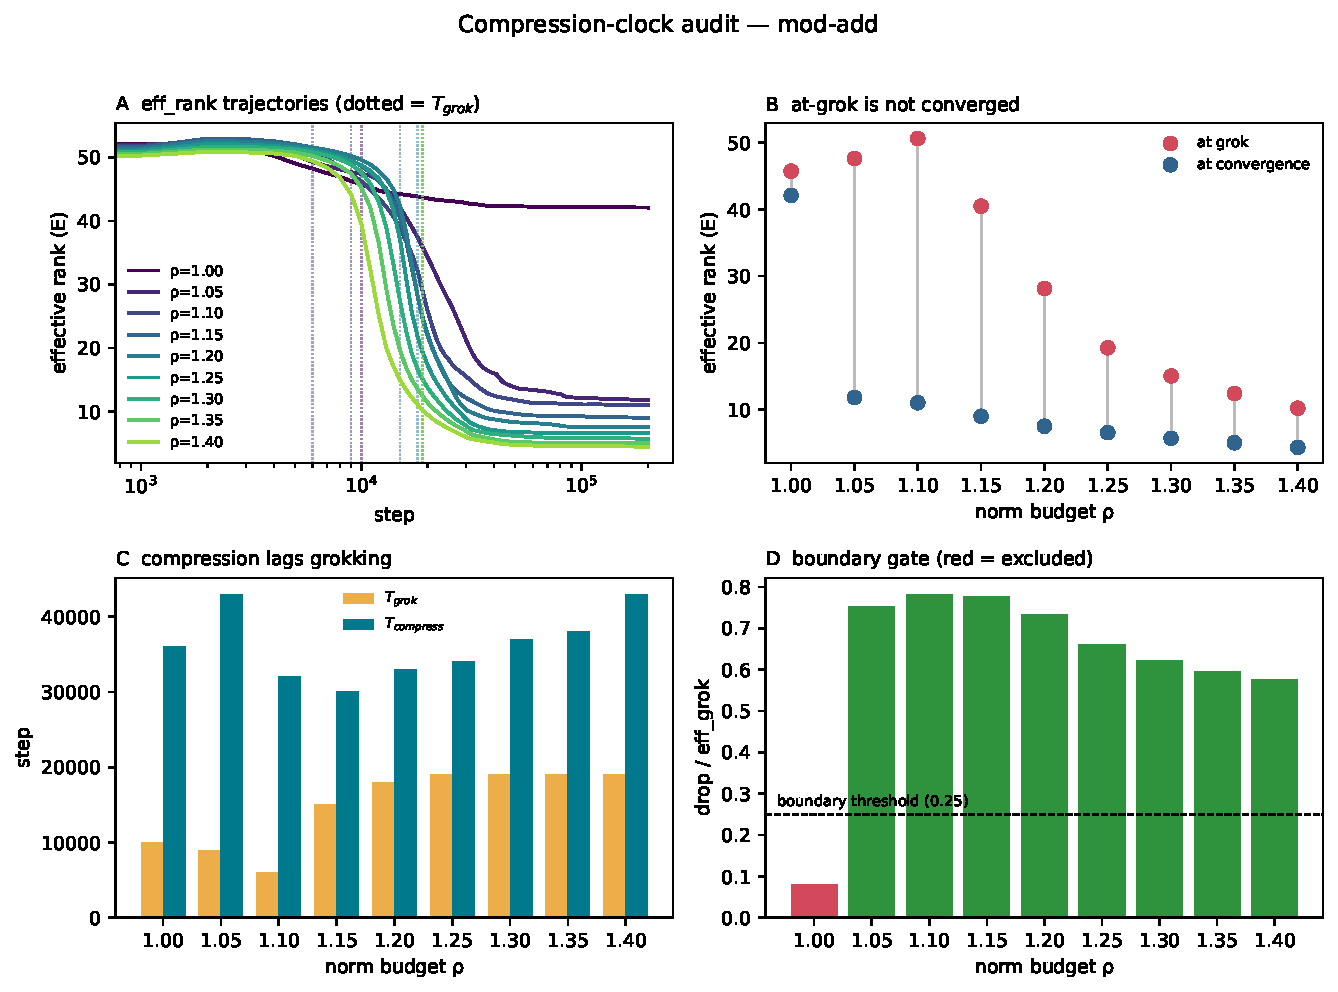
\includegraphics[width=\textwidth]{fig_dashboard_modadd.pdf}
\caption{Compression-lag dashboard on the modular-addition MLP ($p=59$, 6 seeds, real data), the
primary result. \textbf{A}: embedding effective-rank trajectories per norm budget $\rho$ (dotted:
$T_{\mathrm{grok}}$); fast-grokking budgets fall from $\approx\!50$ to a low floor, while the floor cell
$\rho=1.00$ (dark) stays near $42$. \textbf{B}: effective rank at grokking (red) vs.\ at convergence
(blue) --- the at-grok value sits well above the converged floor at every budget that completes, i.e.\ it
is a transient; only at $\rho=1.00$ do the two coincide (no compression). \textbf{C}:
$T_{\mathrm{grok}}$ (orange) vs.\ $T_{\mathrm{compress}}$ (teal); compression lags grokking at every
budget. \textbf{D}: the boundary gate --- the $\rho=1.00$ cell (red) has a drop/at-grok ratio below
threshold and is excluded before the ordering statistics are computed, preventing a spurious two-clock
verdict.}
\label{fig:mlp}
\end{figure}

\paragraph{The concrete failure mode.} Figure~\ref{fig:atgrok} makes the hazard explicit by plotting
the effective rank \emph{read at grokking} against the \emph{converged} floor, both as functions of the
norm budget. The two curves tell qualitatively different stories. The converged curve is the depth law:
a strict monotone fall from the boundary cell down to a low floor. The at-grok curve is high and nearly
flat at the low-budget end, then falls, and at every budget that compresses it sits $3$--$5\times$
above the converged value (median $3.3\times$). Most sharply, the at-grok snapshot cannot separate
the one cell that does not compress from the ones that do: the boundary cell ($\rho=1.00$, converged
rank $\approx\!42$) and its neighbour ($\rho=1.05$, converged rank $\approx\!12$) read $46$ and $48$ at
grok, a $4\%$ difference that hides a $3.6\times$ difference in the converged solution. A study that
read embedding rank at the transition would therefore report a circuit complexity several-fold too high,
miss that one budget never compresses, and recover a complexity-vs-budget shape that the converged
network does not have. This is the failure mode the audit exists to catch; it is not hypothetical, and
it is invisible without training past the transition.

\begin{figure}[!htb]
\centering
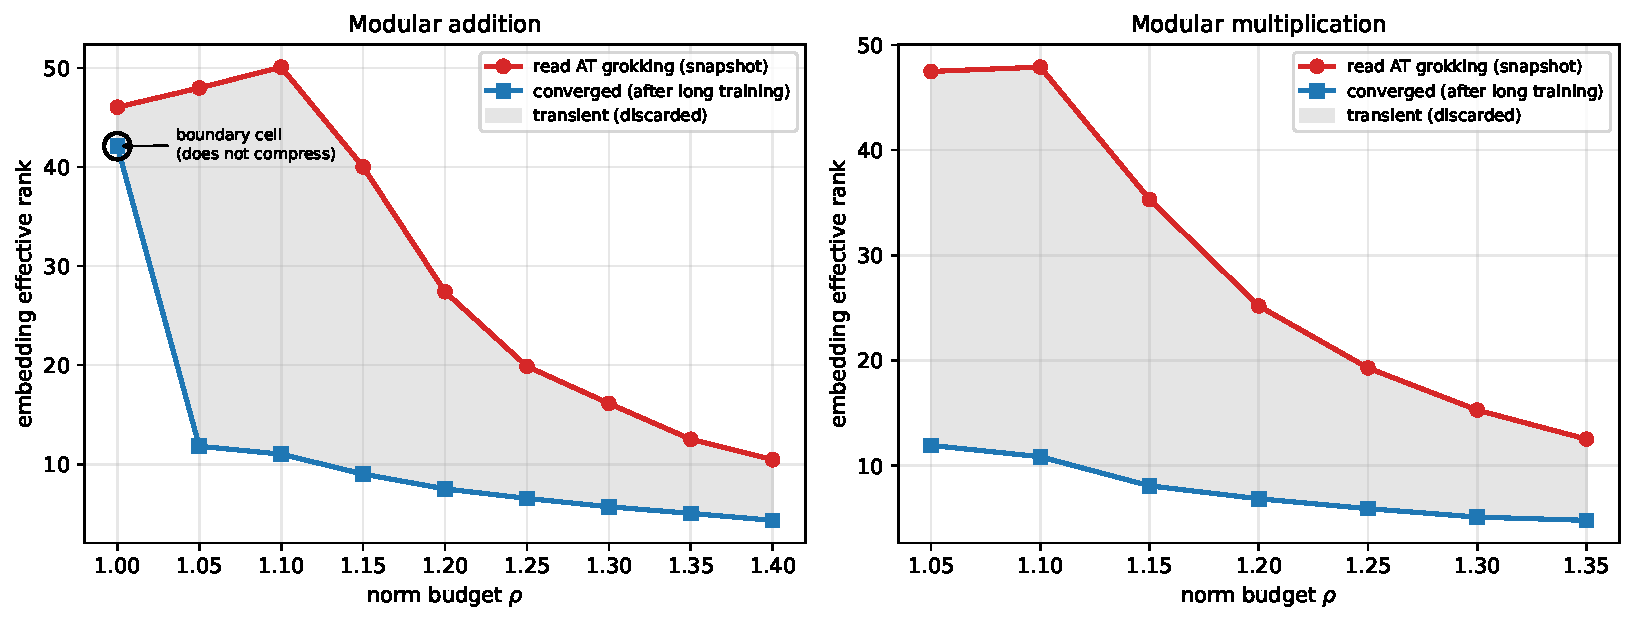
\includegraphics[width=\textwidth]{fig_atgrok_vs_converged.pdf}
\caption{\textbf{Reading effective rank at grokking inverts the picture.} Embedding effective rank read
\emph{at} grokking (red) vs.\ the \emph{converged} floor after long training (blue), against the norm
budget $\rho$; the grey band is the transient the converged network discards. The converged curve is the
monotone depth law; the at-grok curve overstates it by $3$--$5\times$ and is nearly flat where the
converged curve falls steepest. On addition (left) the boundary cell $\rho=1.00$ (circled) reads the same
as its neighbours at grok but never compresses --- a distinction the snapshot erases and only long
training reveals. Regenerated by \texttt{make\_atgrok\_vs\_converged\_figure.py}.}
\label{fig:atgrok}
\end{figure}

\paragraph{Not specific to the clamp protocol or to modular arithmetic.} The transient is the paper's
central claim, and it depends on neither the norm-clamp intervention nor modular arithmetic. On a
free weight-decay sweep at $p=59$, with no norm clamp at all, the at-grok embedding rank exceeds
the converged floor in every fully-generalizing cell on modular addition (median $37\!\to\!18$),
modular multiplication ($35\!\to\!18$), and parity, a non-arithmetic task ($23\!\to\!3$): a
$2$--$7\times$ overstatement, with parity showing the largest transient (\texttt{transient\_replication.py}).
The transient is also metric-agnostic. On the same free-decay addition cells the at-grok
overstatement appears in participation ratio ($2.2\times$) and stable rank ($1.4$--$1.7\times$) just as in
effective rank ($2.5$--$2.6\times$), and the one decay setting with no effective-rank transient shows none
in the other two either, so the hazard is a property of the representation's spectral compression rather than
of the particular rank measure (\texttt{metric\_agnostic\_transient.py}).
One thing does not carry over, and we flag it rather than bury it: the depth law's direction.
Under the clamp protocol the converged floor falls with the norm budget; under free weight decay it
\emph{rises} with the decay strength, and the two do not collapse onto a single floor-versus-converged-norm
curve (\S\ref{sec:limitations}). The transient generalizes across protocol and task; the depth law's sign
is protocol-specific.

\section{Generalization precedes compression: a large lag}
On both modular addition and multiplication the audit returns \textsc{partially separated clocks + large
lag} (Table~\ref{tab:clocks}). Compression follows grokking by a lag comparable to the time-to-grok
itself: median lag $1.7\times10^4$ steps on multiplication ($\mathrm{lag}/T_{\mathrm{grok}}=1.04$) and
$1.8\times10^4$ on addition ($\mathrm{lag}/T_{\mathrm{grok}}=1.00$); Figure~\ref{fig:mlpmult} is the
multiplication dashboard. This large separation is the robust,
replicated result. The norm budget strongly orders $T_{\mathrm{grok}}$
($\rho_S(\rho,T_{\mathrm{grok}})=+0.90,+0.85$) but does \emph{not} order $T_{\mathrm{compress}}$
($\rho_S(\rho,T_{\mathrm{compress}})=+0.18,+0.29$): generalization onset and representation compression
are temporally separable, with a real and large gap, but the compression time is not a clean function of
the budget. We therefore report a large separation rather than a single shared clock.

\begin{table}[!htb]
\centering
\small
\caption{Compression-lag audit on the two modular-arithmetic MLPs ($p=59$, 6 seeds per cell,
$2\times10^5$-step budget), on the enlarged budget grid. The large post-grok lag and the
monotone floor law replicate on both tasks; the compression \emph{time} is not cleanly ordered by the
budget. On modular addition the boundary gate excludes the floor cell $\rho=1.00$, which only partially
generalizes and never compresses, before the ordering statistics are computed.}
\label{tab:clocks}
\begin{tabular}{lcc}
\toprule
 & modular multiplication & modular addition \\
\midrule
cells (norm budgets $\rho$) & 7 ($1.05$--$1.35$) & 9 ($1.00$--$1.40$) \\
median gap $T_{\mathrm{compress}}-T_{\mathrm{grok}}$ & $17{,}000$ & $18{,}000$ \\
$\mathrm{lag}/T_{\mathrm{grok}}$ & $1.04$ & $1.00$ \\
$\rho_S(\rho,T_{\mathrm{grok}})$ & $+0.90$ & $+0.85$ \\
$\rho_S(\rho,T_{\mathrm{compress}})$ & $+0.18$ & $+0.29$ \\
$\rho_S(\rho,\text{converged floor})$ & $-1.00$ & $-1.00$ \\
boundary cell excluded & --- & $\rho=1.00$ \\
verdict & partially separated + large lag & partially separated + large lag \\
\bottomrule
\end{tabular}
\end{table}

\begin{figure}[!htb]
\centering
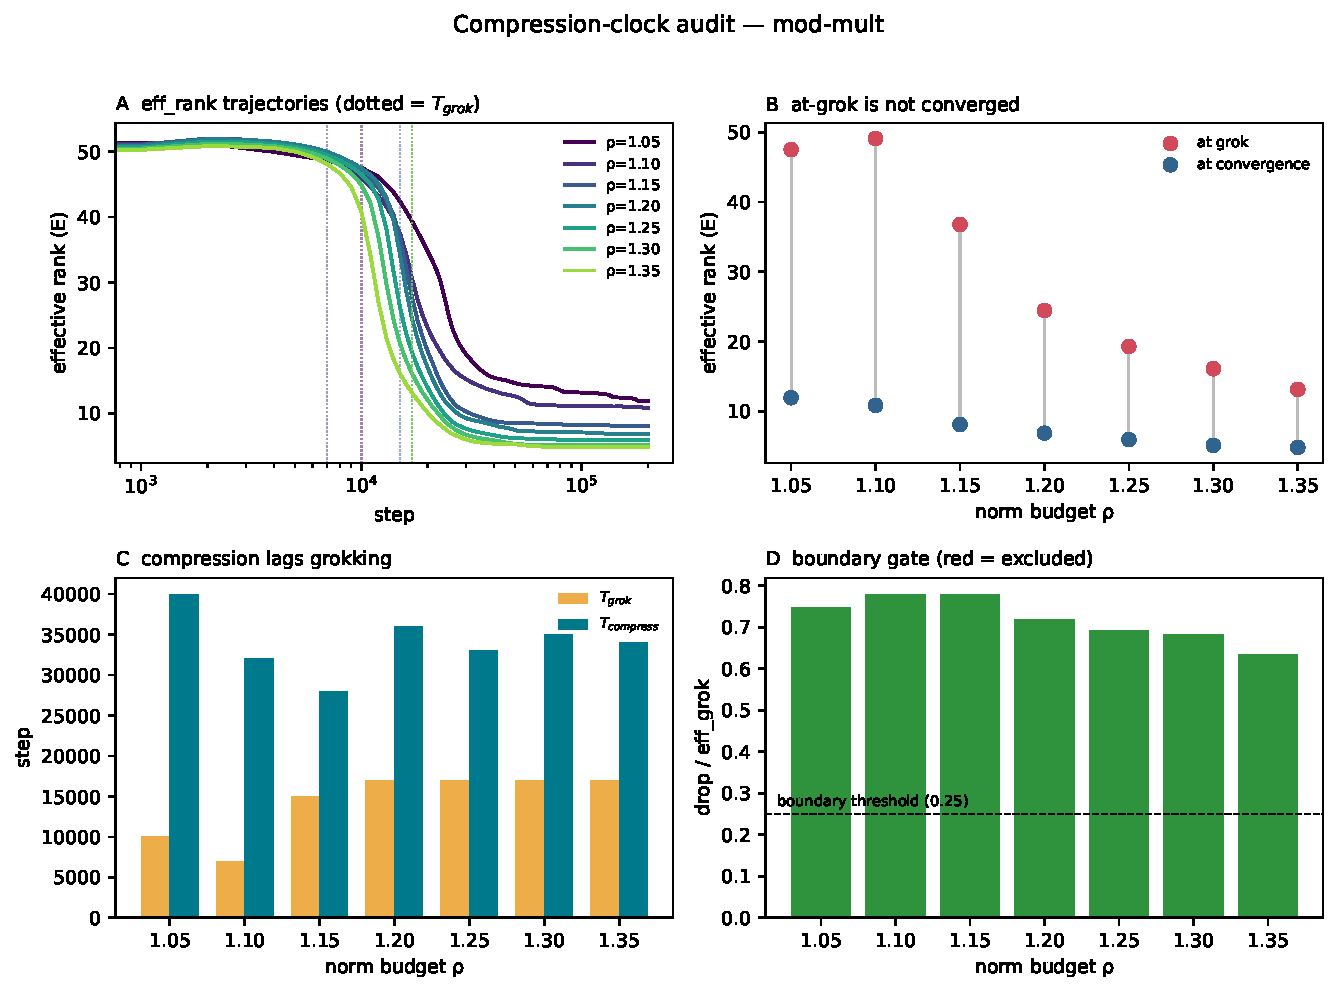
\includegraphics[width=\textwidth]{fig_dashboard_modmult.pdf}
\caption{The same audit on the modular-multiplication MLP ($p=59$, 6 seeds, real data), a replication of
Figure~\ref{fig:mlp}. The at-grok transient (B) and the compression lag (C) recur; here the swept budgets
($\rho=1.05$--$1.35$) all lie above the functional floor, so all cells compress and none is gated (D).
The post-grok lag is comparable to $T_{\mathrm{grok}}$ on both tasks
($\mathrm{lag}/T_{\mathrm{grok}}=1.04$ here vs.\ $1.00$ on addition), illustrating that the same
qualitative separation recurs with a task-specific coefficient.}
\label{fig:mlpmult}
\end{figure}

\paragraph{What the norm budget controls on the MLP: the depth of compression.} The budget's clean effect
here is not on when compression finishes but on how far it goes: the converged
effective-rank floor decreases monotonically with $\rho$ ($\rho_S(\rho,\text{floor})=-1.0$ at both tasks,
bootstrap $95\%$ CI $[-1.0,-1.0]$ on addition and $[-1.0,-0.93]$ on multiplication), and the rank read
at grokking is itself lower at higher budgets ($\rho_S\approx-0.97$). This explains the weak
ordering of $T_{\mathrm{compress}}$: a higher-budget cell groks later but starts post-grok compression
from an already-lower rank with less distance to fall. We do not over-read this depth law. It is an
MLP-specific regularity that does not survive a change of architecture, as the transformer sweep
below shows (\S\ref{sec:transformer}, Fig.~\ref{fig:depthlaw}), and we report it as a scoped observation
rather than a norm law.

\paragraph{A corrected reading.} An earlier, smaller grid (four and five budget cells) showed
same-signed $T_{\mathrm{compress}}$ correlations ($+0.40$ and $+0.95$) that invited a ``one clock''
reading. Enlarging the grid to seven and nine cells weakened that ordering sharply --- the
multiplication $T_{\mathrm{compress}}$ correlation fell to $+0.18$ and addition to $+0.29$, neither an
ordering --- while leaving the large lag and the floor law intact. We report this openly: it is the same
standard the audit enforces against others, that a correlation on four points is not an ordering,
applied to our own earlier reading. Both readings are reproducible: \texttt{corrected\_reading.py}
recomputes $\rho_S(\rho,T_{\mathrm{compress}})$ on the small grid ($+0.95$ addition, $+0.40$
multiplication) and the full grid ($+0.29$, $+0.18$) from the data shipped in \texttt{sample\_data/}.


\paragraph{Why the boundary gate matters.} If the partially-generalizing floor cell is left in, its
high, never-compressing rank produces a degenerate $T_{\mathrm{compress}}$ that, combined with the
genuine cells, can flip the global ordering and yield a false \textsc{two clocks} verdict. On modular
addition this is concrete: the $\rho=1.00$ cell sits at effective rank $42.1$ at convergence (versus a
typical floor of $7.5$ for the cells that complete), a drop of only $0.09$ relative to its at-grok
value, since it groks only partially and never compresses. The audit detects such cells by their tiny
drop-to-at-grok ratio and high floor, excludes them from the dose-response, and reports them
separately as boundary cells. This single guard is the difference between a fragile finding and a
robust one.

\paragraph{Relation to topological accounts.} \citet{tang2026topological} report that, for MLPs,
test accuracy precedes the persistent-homology transition by only $\sim\!10^3$ steps (a near-synchronous
cross-correlation lag), with LID compression in the same window. Our rank-compression lag is
$\sim\!2\times10^4$ steps. We flag this gap cautiously: the two numbers come from different setups
(task, prime, model, and lag definition all differ), so a direct ratio is suggestive at best. What it
motivates is a clean experiment rather than a conclusion: measuring persistent homology, LID, and effective
rank on the same runs to test whether topological reorganization and rank compression are one
event or two. We state the distinctness only as a hypothesis; the audit makes the rank clock easy to
place alongside the others when that experiment is run.


\paragraph{Robustness to the audit's free parameters.} The audit exposes five thresholds: the
compression fraction $\varepsilon$, the floor-averaging window, the grokking accuracy threshold, the
minimum at-grok drop, and the boundary drop-threshold. Table~\ref{tab:sensitivity} varies each one at a
time, holding the rest at their defaults. Three findings are invariant across \emph{every} setting: the
converged floor law is Spearman $-1.0$ on both tasks; the boundary gate excludes exactly the $\rho=1.00$
cell on addition and no cell on multiplication; and the large post-grok lag is always retained while the
$T_{\mathrm{grok}}$/$T_{\mathrm{compress}}$ ordering never flips to opposite-signed --- so the verdict
never collapses to a \emph{coincident} (zero-lag) shared clock and never becomes two oppositely-ordered
clocks. In $28$ of the $30$ settings the verdict is \textsc{partially separated + large lag}; in $2$
($\varepsilon=0.20$ on multiplication and $\mathrm{grok\,thr}=0.99$ on addition) the same-signed ordering
is strong enough that the analyzer labels it \textsc{one clock + large lag}, i.e. a single ordering with
the lag still present, not a coincident clock --- the verdict family is stable even where the label
crosses that threshold. The one
quantity that moves is the lag coefficient: $\mathrm{lag}/T_{\mathrm{grok}}$ ranges over $[0.65,1.46]$ as
$\varepsilon$ varies from $0.20$ to $0.05$, because $\varepsilon$ sets how close to the floor counts as
``compressed.'' The lag magnitude stays of order $T_{\mathrm{grok}}$ ($\geq\!10^4$
steps) throughout; only its calibration moves. We report $\varepsilon=0.10$ (where
$\mathrm{lag}/T_{\mathrm{grok}}\approx1.0$) as the default and note that this dependence is monotone and
expected, not a sign of fragility.

\begin{table}[!htb]
\centering
\footnotesize
\caption{\textbf{Sensitivity of the audit to its free parameters} (full grid; each parameter varied one
at a time, the rest held at the defaults $\varepsilon=0.10$, floor frac $0.10$, grok thr $0.90$, min drop
$1.0$, gate thr $0.25$). The converged-floor law $\rho_S(\text{floor})=-1.0$ and the boundary gate
(addition excludes $\rho=1.00$; multiplication excludes none) are invariant across all settings; only the
lag coefficient $\mathrm{lag}/T_g$ moves, tracking $\varepsilon$ as expected. ``gated'' lists the budgets
the boundary gate removes before the ordering statistics are computed. Regenerated by
\texttt{sensitivity\_floor\_ci.py}.}
\label{tab:sensitivity}
% auto-generated by sensitivity_floor_ci.py
\begin{tabular}{llcccccc}
\toprule
parameter & task & gated & lag & lag/$T_g$ & $\rho_S(T_g)$ & $\rho_S(T_c)$ & $\rho_S$(floor) \\
\midrule
$\varepsilon$$=0.05$ & add & 1.00 & 24750 & 1.36 & $+0.85$ & $+0.17$ & $-1.00$ \\
$\varepsilon$$=0.05$ & mult & --- & 25500 & 1.46 & $+0.90$ & $+0.39$ & $-1.00$ \\
$\varepsilon$$=0.1$ & add & 1.00 & 18000 & 1.03 & $+0.85$ & $+0.29$ & $-1.00$ \\
$\varepsilon$$=0.1$ & mult & --- & 17000 & 1.03 & $+0.90$ & $+0.18$ & $-1.00$ \\
$\varepsilon$$=0.2$ & add & 1.00 & 11500 & 0.65 & $+0.85$ & $+0.40$ & $-1.00$ \\
$\varepsilon$$=0.2$ & mult & --- & 10500 & 0.67 & $+0.90$ & $+0.20$ & $-1.00$ \\
\midrule
floor frac$=0.05$ & add & 1.00 & 18000 & 1.03 & $+0.85$ & $+0.29$ & $-1.00$ \\
floor frac$=0.05$ & mult & --- & 17000 & 1.03 & $+0.90$ & $+0.21$ & $-1.00$ \\
floor frac$=0.1$ & add & 1.00 & 18000 & 1.03 & $+0.85$ & $+0.29$ & $-1.00$ \\
floor frac$=0.1$ & mult & --- & 17000 & 1.03 & $+0.90$ & $+0.18$ & $-1.00$ \\
floor frac$=0.2$ & add & 1.00 & 18000 & 1.03 & $+0.85$ & $+0.29$ & $-1.00$ \\
floor frac$=0.2$ & mult & --- & 17000 & 1.03 & $+0.90$ & $+0.18$ & $-1.00$ \\
\midrule
grok thr$=0.9$ & add & 1.00 & 18000 & 1.03 & $+0.85$ & $+0.29$ & $-1.00$ \\
grok thr$=0.9$ & mult & --- & 17000 & 1.03 & $+0.90$ & $+0.18$ & $-1.00$ \\
grok thr$=0.95$ & add & 1.00 & 18750 & 0.97 & $+0.91$ & $+0.31$ & $-1.00$ \\
grok thr$=0.95$ & mult & --- & 17500 & 0.97 & $+0.92$ & $+0.32$ & $-1.00$ \\
grok thr$=0.99$ & add & 1.00 & 20000 & 0.93 & $+0.91$ & $+0.30$ & $-1.00$ \\
grok thr$=0.99$ & mult & --- & 19500 & 0.97 & $+0.98$ & $+0.54$ & $-1.00$ \\
\midrule
min drop$=0.5$ & add & 1.00 & 18000 & 1.03 & $+0.85$ & $+0.29$ & $-1.00$ \\
min drop$=0.5$ & mult & --- & 17000 & 1.03 & $+0.90$ & $+0.18$ & $-1.00$ \\
min drop$=1.0$ & add & 1.00 & 18000 & 1.03 & $+0.85$ & $+0.29$ & $-1.00$ \\
min drop$=1.0$ & mult & --- & 17000 & 1.03 & $+0.90$ & $+0.18$ & $-1.00$ \\
min drop$=2.0$ & add & 1.00 & 18000 & 1.03 & $+0.85$ & $+0.29$ & $-1.00$ \\
min drop$=2.0$ & mult & --- & 17000 & 1.03 & $+0.90$ & $+0.18$ & $-1.00$ \\
\midrule
gate thr$=0.2$ & add & 1.00 & 18000 & 1.03 & $+0.85$ & $+0.29$ & $-1.00$ \\
gate thr$=0.2$ & mult & --- & 17000 & 1.03 & $+0.90$ & $+0.18$ & $-1.00$ \\
gate thr$=0.25$ & add & 1.00 & 18000 & 1.03 & $+0.85$ & $+0.29$ & $-1.00$ \\
gate thr$=0.25$ & mult & --- & 17000 & 1.03 & $+0.90$ & $+0.18$ & $-1.00$ \\
gate thr$=0.3$ & add & 1.00 & 18000 & 1.03 & $+0.85$ & $+0.29$ & $-1.00$ \\
gate thr$=0.3$ & mult & --- & 17000 & 1.03 & $+0.90$ & $+0.18$ & $-1.00$ \\
\bottomrule
\end{tabular}

\end{table}

\section{Why a tested audit, and not just a metric}
The case for this paper is not a new metric, since effective rank is borrowed, but the claim that
measurement reliability is itself a result in a literature that increasingly reads structure off single
transition-time snapshots. We make that case concretely. The audit is built around explicit failure modes
rather than a happy path. It (i) flags censoring when cells do not reach the compression
threshold within budget; (ii) excludes boundary/incomplete-grok cells before any ordering statistic is
computed; (iii) emits \textsc{low-power / descriptive only} when fewer than two non-boundary cells
remain; and (iv) returns \textsc{large lag, ordering undetermined} --- rather than asserting a shared
clock --- whenever the order statistic across budgets is undefined (too few cells or tied values).
Each of these is a verdict the tool will return \emph{against} a tidy conclusion when the data do not
support one; in our own modular-multiplication data the weak ($+0.40$) ordering is exactly the regime
where this restraint matters.

\paragraph{The audit caught its own author.} The strongest evidence that these checks are load-bearing is that they fired on us. During development
a reporting branch that added genuinely useful low-power and no-grok diagnostics was forked from before
two ordering fixes, and it re-introduced a verdict that asserted ``one clock'' while the underlying rank
correlation was undefined ($\mathrm{NaN}$ Spearman). The nine-case adversarial suite caught this, not
because a verdict string was missing, but because the suite requires a clock-type verdict to be backed by
a finite order statistic. A test that checked only for the presence of the words ``one clock'' would have
passed the broken analyzer; its own bundled test did. This is one way a representation study can fool
itself, with a measurement that looks like a finding but rests on an undefined or transient quantity. The
same check fired a second time at the data level: an initial four- and five-cell grid showed same-signed
$T_{\mathrm{compress}}$ ordering that read as a single clock, and enlarging the grid to seven and nine
cells dissolved it, which is the ``a correlation on a handful of points is not an ordering'' failure the
audit is built to flag. We report the corrected reading rather than the original.

\paragraph{Adversarial test suite.} The suite ships nine pre-registered cases: clean one-clock,
all-censored, high-floor boundary, true two-clock, single-valid-cell, non-monotone (rank rebounds after
falling), compression-before-grok, tied orderings, and heavy noise. Each case fixes the expected verdict
\emph{and the reason} before running; a case that passes only by avoiding a crash is treated as a
failure. The suite, the analyzer, an adapter for externally-logged runs, sample data, and the figure
generator are released so that the audit can be run on other studies' trajectories.

\section{A transformer dose-response, and a depth-law ablation}
\label{sec:transformer}
The MLP results above raise two questions that the same intervention can answer on a second
architecture: does the at-grok transient, the paper's central claim, generalize, and does the norm-budget
depth law generalize? We therefore run a well-powered transformer sweep to true convergence, a one-layer
un-normalized attention model on modular addition ($p=59$), under both the clamp protocol (seven budgets
$\rho\in[0.9,1.4]$) and a free weight-decay protocol (six decays), three seeds each, with dense post-grok
logging of five spectral measures at four weight loci and the activation representation. The two
questions settle in opposite directions.

\paragraph{The central claim generalizes: the transient is architecture-independent.}
On the clamp sweep, the embedding effective rank read at grokking sits above its converged floor in
$92\%$ of generalizing, non-censored cells (median $1.34\times$); the unembedding overstates by
$1.48\times$ in every such cell, and the free-decay sweep shows the same ($1.36\times$ and $1.38\times$;
Fig.~\ref{fig:tftransient}). The overstatement is metric-agnostic, appearing in Roy-Vetterli
and variance-normalized effective rank, participation ratio, and stable rank alike, and present at
every locus we log: it is largest on the MLP-block output weights ($W_{\mathrm{out}}$, up to
$3.6\times$ at the smallest budget), confirming that the hazard is a property of representation
compression rather than of one matrix or one measure. As on the MLP, the size of the transient is set by
the budget (largest at small $\rho$, shrinking toward the high-budget cells). The magnitude is more
modest than the $3$--$5\times$ overstatement of the modular MLP: on the transformer the embedding
transient is $\approx\!1.3$--$1.5\times$. We report it for what it is, a smaller but robust and now
architecture-general measurement hazard, and do not inflate the headline magnitude.

\begin{figure}[!htb]
\centering
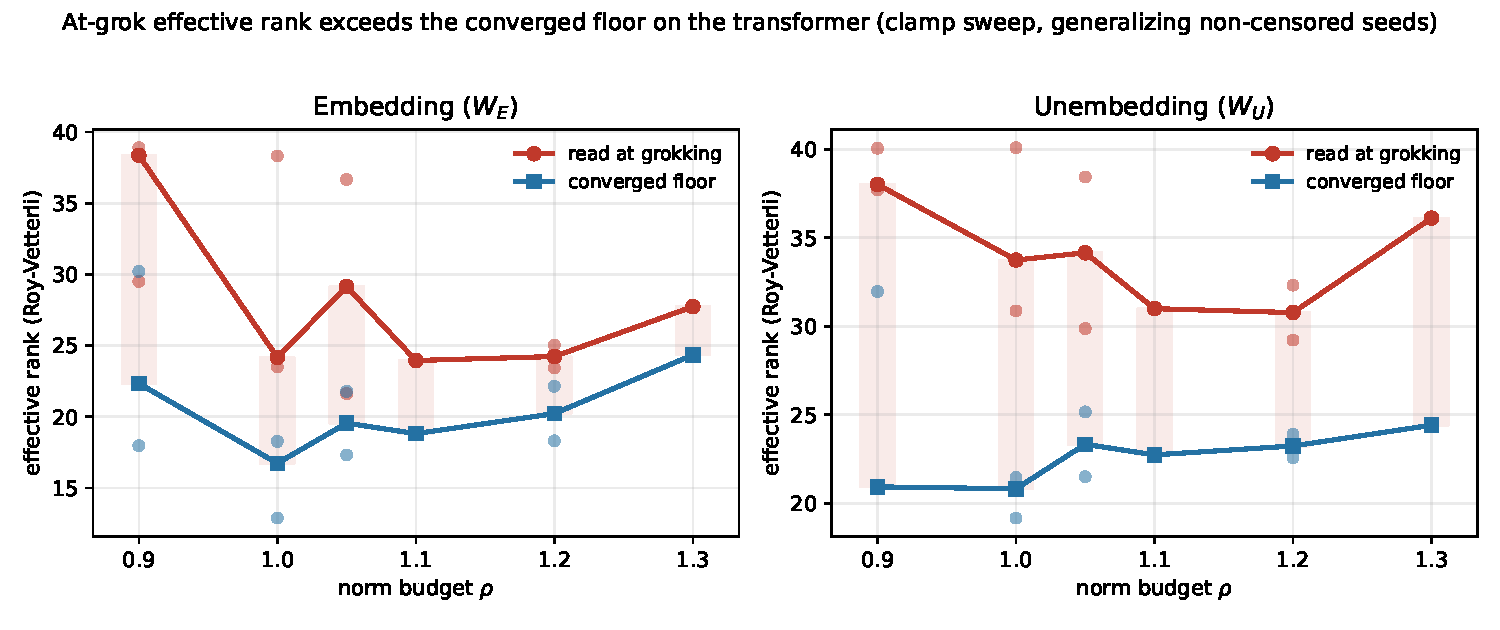
\includegraphics[width=\textwidth]{fig_transformer_transient.pdf}
\caption{\textbf{The at-grok transient generalizes to the transformer.} Effective rank (Roy-Vetterli)
read \emph{at} grokking (red) vs.\ the \emph{converged} floor (blue) across the clamp norm budget $\rho$,
for the embedding $W_E$ (left) and unembedding $W_U$ (right); points are generalizing, non-censored seeds
and lines are per-budget medians, with the transient shaded. The at-grok value sits above the converged
floor at almost every budget on both loci (median $1.34\times$ on $E$, $1.48\times$ on $U$), reproducing
the modular-MLP transient on a different architecture at a smaller magnitude. Regenerated by
\texttt{transformer\_sweep\_audit.py}.}
\label{fig:tftransient}
\end{figure}

\paragraph{The lag recurs.} The post-grok compression lag also transfers: across the clean transformer
cells the median lag is $\approx\!2.7\times10^4$ steps ($\mathrm{lag}/T_{\mathrm{grok}}\approx0.63$), and
as on the MLP the compression time is not cleanly ordered by the budget
($\rho_S(\rho,\mathrm{lag})=+0.37$, $p=0.47$, $n=6$ cells --- a low-power estimate, since several clean
cells rest on a single generalizing seed, so we read it as a non-ordering rather than a precise
coefficient). The large-but-not-budget-ordered separation of generalization onset from representation
compression is thus a consistent two-architecture finding. This lag is computed by the same per-seed
clock as the MLP audit, restricted to the generalizing, non-censored clamp cells.

\paragraph{The depth law does \emph{not} generalize: a negative result.} The norm-budget depth law is a
different story, and we report the negative result plainly. On the transformer the converged floor does
not fall with the budget at any weight or activation locus we log: on the embedding it is essentially
unordered ($\rho_S(\rho,\text{floor})=+0.14$, $p=0.66$, non-censored generalizing cells), on the
unembedding weakly positive ($+0.42$, n.s.), and on the activation representation significantly positive
($+0.82$, $p<0.01$). Where the modular MLP shows a strict monotone fall ($-1.0$;
Fig.~\ref{fig:depthlaw}), the transformer floor is flat or, on the activation locus, ordered in the
opposite direction. The negative result therefore does not hinge on a single non-significant null
on one matrix: it is a consistent failure of the monotone fall across three loci, one of which reverses
the sign outright. We checked that this is not a censoring artifact: high-budget cells grok late
and were excluded if their floor was still falling at the step cap, and the result holds on the cells that
remain. Combined with the protocol reversal already noted on the MLP (free weight decay orders the floor
oppositely to the clamp), this establishes that the depth law is specific to the modular-arithmetic MLP
and does not survive a change of architecture. The standard that motivates this paper applies to its own
secondary result: a clean dose-response on one architecture is not a law until it is shown on another, and
here it is not.

\begin{figure}[!htb]
\centering
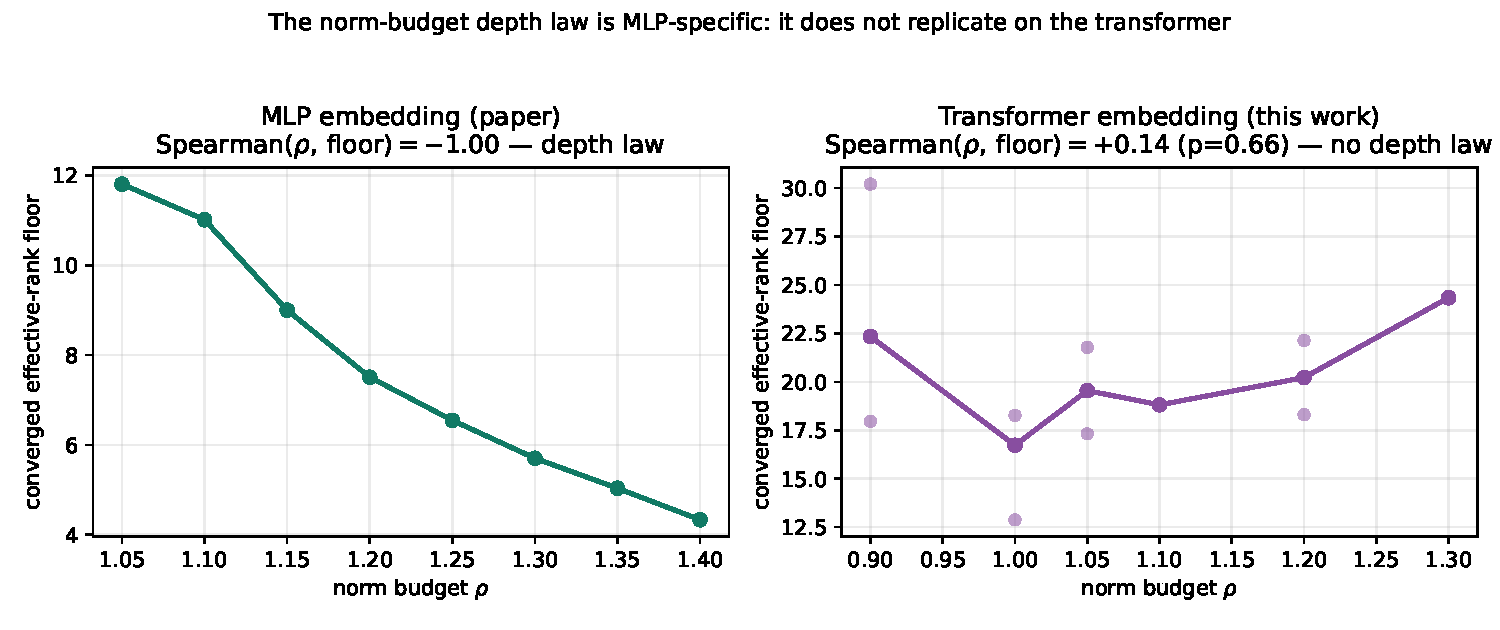
\includegraphics[width=\textwidth]{fig_depthlaw_nonreplication.pdf}
\caption{\textbf{The norm-budget depth law is MLP-specific (negative result).} Converged effective-rank
floor vs.\ the clamp norm budget $\rho$. \textbf{Left}, the modular-addition MLP (paper data): the floor
falls monotonically, Spearman $-1.0$ --- the depth law. \textbf{Right}, the transformer embedding (this
work, non-censored generalizing seeds): the floor does not fall, Spearman $+0.14$ ($p=0.66$). The
relationship that looked like a law on the MLP does not replicate on a second architecture. Regenerated by
\texttt{transformer\_sweep\_audit.py}.}
\label{fig:depthlaw}
\end{figure}

\paragraph{Generalization is seed-fragile here, and we flag it.} The un-normalized transformer groks
erratically across seeds at this configuration: only $16$ of $21$ clamp cells and $14$ of $18$ free-decay
cells reach $0.90$ test accuracy, with grok times for the same budget ranging from $\sim\!10^3$ to
$>\!10^5$ steps and one seed failing to grok at all. We therefore restrict every transformer statistic
above to cells that fully generalize and whose floor has plateaued, and we report the transformer as a
generalization check on the transient (which passes) and a generality test of the depth law (which
fails), not as a clean second dose-response.

\section{Architecture generality of the transient, and where the lag comes from}
\label{sec:arch}
The central claim is established on the modular MLP and, in \S\ref{sec:transformer}, on a transformer
under the clamp. To test whether it depends on being a transformer, on attention, on
normalization, or on initialization, which differ all at once between the two, we run a single
free-weight-decay harness that changes one thing at a time: arm A is the MLP anchor; arm B is a canonical
attention model that is LayerNorm-free (ReLU MLP block, no biases, $1/\sqrt{d}$ initialization); arm C is
arm B with LayerNorm added and nothing else. A-vs-B isolates architecture; B-vs-C isolates LayerNorm.
Each arm is swept under free weight decay (MLP $\{0.5,1,2,4\}$; transformer $\{1,1.5,2,3\}$), $p=59$,
train fraction $0.3$, up to $6\times10^4$ steps, every quantity computed by the same per-seed clock as the
MLP audit.

\paragraph{The transient is architecture-general.} The at-grok transient exceeds the converged floor on
all three arms: $\approx\!1.5\times$ on the MLP, $\approx\!1.5\times$ on the canonical transformer, and
$\approx\!3.2\times$ on the LayerNorm transformer. As on the modular MLP, reading embedding rank at the
transition overstates the converged value on every architecture we tried; the hazard is not specific to
the MLP or to the clamp.

\paragraph{What the lag depends on: how much compression precedes grokking.} The arms differ sharply in
when the embedding compresses relative to grokking. Define $\mathrm{frac\text{-}pre} =
(r_{\mathrm{init}}-r_{\mathrm{grok}})/(r_{\mathrm{init}}-r_{\mathrm{floor}})$, the fraction of the total
embedding-rank compression already completed by the grok step. It is $0.87$ on the canonical transformer
(almost all compression precedes grokking, leaving a near-zero lag and a small transient), $0.66$ on the
MLP, and $0.25$ on the LayerNorm transformer (most compression follows grokking, producing both the large
lag and the $\approx\!3\times$ transient). The single LayerNorm ablation B-vs-C moves frac-pre from $0.87$
to $0.25$: within this harness it is LayerNorm, not ``being a transformer,'' that defers compression past
grokking. Equivalently, the grok-to-compression lag is near-concurrent for the canonical transformer and
large only with LayerNorm or on the MLP. We read the lag qualitatively here, since its precise coefficient is
seed-sensitive when a high frac-pre leaves only a narrow band to the floor, and note that its
direction agrees with the better-powered transformer estimate of \S\ref{sec:transformer}
($\mathrm{lag}/T_{\mathrm{grok}}\approx0.63$). The transient and the lag are thus two views of one
quantity, how much of the representation has compressed at the moment one reads it; the normalization
scheme sets that quantity. Consistent with this, the post-grok coupling between the global weight norm and
the embedding rank is strongly negative only under LayerNorm (Spearman $-0.80$) and positive for the
canonical model ($+0.70$): the LayerNorm arm compresses as its norm grows after grokking, whereas the
canonical arm has already compressed.

\paragraph{A second non-stationarity: the floor itself need not be stable.} The low-budget MLP cells
($wd=0.5$) expose a separate hazard that sharpens the paper's thesis. There the embedding groks at rank
$\approx\!22$, holds a plateau, and then, well after grokking, undergoes a second transition in which
the global weight norm roughly doubles and the rank collapses to $\approx\!4$ (Fig.~\ref{fig:arch}C). The
converged floor, computed over the final tenth of training, is read inside this second regime, so a naive
floor is itself transient for these cells. The same failure the audit is built to catch on the at-grok
reading can therefore recur on the denominator: a careful audit must verify that the floor has plateaued,
not merely that training has run long.

\paragraph{What this revises.} This harness refines the transformer lag of \S\ref{sec:transformer} rather
than overturning it: that section's un-normalized model is arm B here, and its low-power lag estimate
agrees in direction with the frac-pre ordering measured here: a canonical transformer compresses at or
near grokking, not long after it. The ``large lag comparable to $T_{\mathrm{grok}}$'' that the MLP shows
(\S\ref{sec:atgrok}) and that a LayerNorm transformer shows is therefore normalization-mediated, not a
property of grokking as such. The audit's job is unchanged: report the separation that exists and name the
variable, normalization, that the data identify, without universalizing a coefficient that the
present data do not pin down.

\begin{figure}[!htb]
\centering
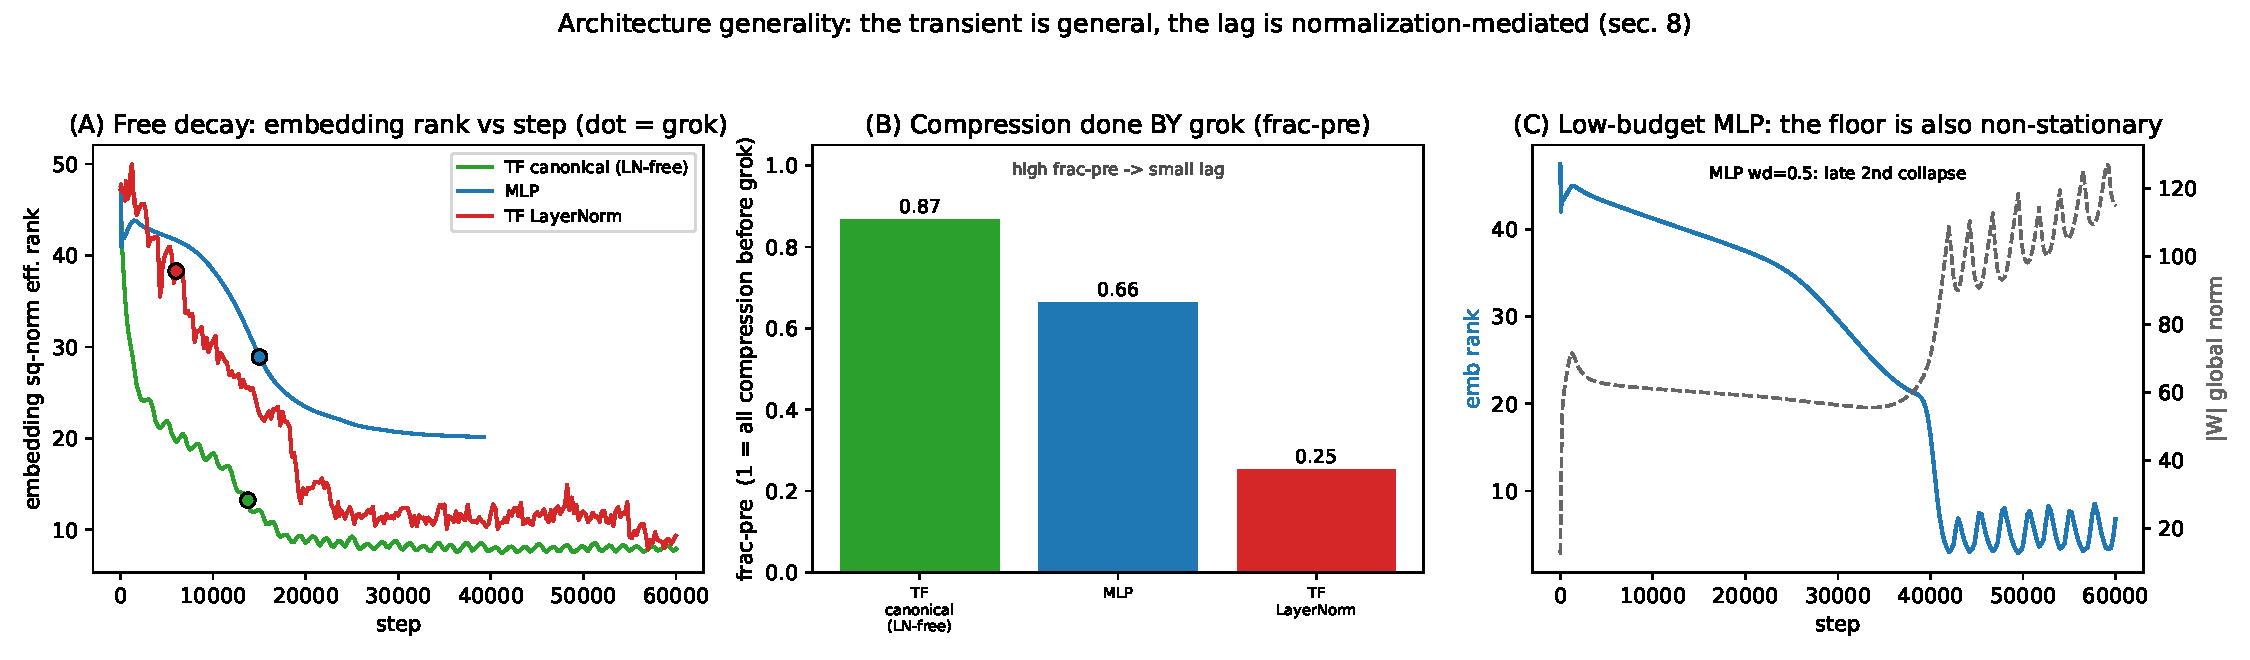
\includegraphics[width=\textwidth]{fig_one_harness_three_arch.pdf}
\caption{\textbf{One harness, three architectures, one variable at a time.} Embedding squared-normalized
effective rank under free weight decay, $p=59$. \textbf{(A)} Representative rank trajectories with the grok
step marked (dot): the canonical transformer (green) has compressed almost entirely by grokking, the
LayerNorm transformer (red) compresses after grokking, and the MLP (blue) is intermediate. \textbf{(B)}
Fraction of the embedding-rank compression completed by the grok step (frac-pre): $0.87$ canonical, $0.66$
MLP, $0.25$ LayerNorm --- the single quantity that orders the arms, and equivalently sets whether the lag
is near-zero or large. \textbf{(C)} A low-budget MLP cell ($wd=0.5$): after grokking the global norm
doubles and the rank undergoes a second, late collapse, so the final-tenth ``floor'' is itself transient.
Regenerated by \texttt{arch\_generality\_audit.py}.}
\label{fig:arch}
\end{figure}

\paragraph{An open mechanism, and the pre-registered test for it.} Why LayerNorm defers compression and
the canonical transformer does not is left open here. A natural hypothesis is scale invariance: LayerNorm
makes the network invariant to the scale of its inputs, so it can reach correct predictions while the
embedding is still high-rank, deferring compression to a later, norm-driven phase. Because this is exactly
the kind of mechanism one can talk oneself into after the fact, we do not assert it. Instead we
provide a pre-registration (\texttt{specs/PREREGISTRATION\_scale\_inv.json}) and an analyzer
(\texttt{audit/analyze\_scale\_invariance.py}) that fix the falsifier in advance: the control arm is the
canonical model with RMS-normalization on the embedding input only (per-token scale invariance and nothing
else), and the account is to be accepted iff a deferral prediction (frac-pre below a fixed threshold) and a
norm-driven prediction (negative post-grok norm--rank coupling) both hold. Running that control, which
requires only adding one arm to the harness, is the clean next step the toolkit is built to support, and we
report the mechanism as a pre-registerable question rather than a result.

\section{Takeaways and future development}
\paragraph{Takeaways.} (1) On modular arithmetic, embedding effective rank at grokking is a
transient, and not only in effective rank: participation ratio and stable rank show the same
overstatement, and the transient also carries to a transformer on both the embedding and the
unembedding (\S\ref{sec:transformer}). The converged network is low-rank at every budget that fully
generalizes, so a single transition-time snapshot can misrepresent the converged circuit. (2) Rank compression does not coincide
with the accuracy transition (contra a common reading) but lags it by an amount of order
$T_{\mathrm{grok}}$ on the MLP. The existence of a separation is the robust, replicated effect, while its magnitude depends on normalization, near-concurrent for a canonical transformer and large only with LayerNorm or on the MLP (\S\ref{sec:arch}). (3) The
norm budget strongly orders $T_{\mathrm{grok}}$ but not $T_{\mathrm{compress}}$. A secondary
observation, which we hold to a higher bar and then break ourselves, is that on the MLP the budget sets,
almost deterministically, the depth of compression (converged effective-rank floor Spearman
$-1.0$); but this depth law is MLP-specific (a transformer clamp sweep trained to convergence does not
reproduce it, $+0.14$ vs.\ $-1.0$; \S\ref{sec:transformer}) and protocol-specific (free weight decay
orders the floor oppositely; \S\ref{sec:limitations}), so we report it as a negative result on generality
rather than a norm law. (4) Measurement reliability is demonstrable, not
assumed: the audit's adversarial suite caught a real false-confidence regression in the analyzer, and
the enlarged grid corrected our own earlier ordering reading, so the check applies to its authors. (5) The deferral mechanism is left open and made testable: we pre-register a scale-invariance control (\S\ref{sec:arch}) and ship its analyzer, rather than asserting a mechanism the present data do not pin down.

\paragraph{Future development of the toolkit.} Several extensions are natural and low-cost.
\emph{Same-run multi-clock measurement}: add persistent-homology, LID, and Fourier-Gini clocks to the
analyzer so the rank, topology, and feature clocks are placed on one timeline from a single run, the
experiment that would turn our rank-vs-topology hypothesis into a result. \emph{Checkpoint-density
guidance}: a planned ablation that subsamples post-grok checkpoints to report how many are needed for a
reliable $T_{\mathrm{compress}}$, turning the transformer censoring we observed into a concrete logging
recommendation. \emph{Metric-agnostic clocks}: the at-grok transient is already metric-agnostic, appearing in
participation ratio and stable rank as well as effective rank (\S\ref{sec:atgrok}), and since the clock
definition needs only a quantity that falls as the representation compresses, running the full lag
measurement under each of these measures is a direct extension; the analyzer's input schema accepts any
such quantity. \emph{Locus selection on transformers}: promote the
two-point E-vs-U locus check into a full per-locus clock, since the right compression locus on a
transformer may be the unembedding rather than the embedding. \emph{Forward/backward coupling}: pairing
the audit with a forward detector \citep{wang2026spectral,xu2026earlywarning} would let a pipeline both
predict a transition and certify whether a measurement taken at it has converged. \emph{Does any
budget-to-floor relation survive scale?} The monotone budget-to-floor relation is established on a small
modular MLP, and the first
generality test, a second architecture, already comes back negative (\S\ref{sec:transformer}).
Whether any budget-to-floor relation reappears on the larger, non-modular systems where rank minimization
has been shown to operate (VGG, U-Net, LSTM, language-model transformers; \citealp{yunis2024spectral})
and across the model scales over which weight decay structures grokking regimes ($0.82$--$85$M;
\citealp{verma2026weightdecay}) is open; given the transformer negative we expect any such relation to be
architecture-dependent rather than a single norm law. The audit's third-party adapter is built to run
that test on others' checkpoints without re-training.

\section{Limitations}
\label{sec:limitations}
The full compression-lag dose-response is established on the MLP (two tasks, seven and nine norm
budgets); on the enlarged grid the compression time is not ordered by the norm budget
($\rho_S(\rho,T_{\mathrm{compress}})=+0.18,+0.29$), so we report the large lag (robust and
architecture-general) and the monotone floor law (robust on the MLP, but architecture-specific as below)
as the two MLP findings, and explicitly do not claim a single shared clock. The depth law itself is
established only on a small modular MLP at one width and is, at most, a modular-MLP-specific echo of a
qualitative observation of \citet{yunis2024spectral} rather than a general quantification of it; it does
not generalize across architecture, since a transformer clamp
sweep trained to convergence shows no monotone floor law (\S\ref{sec:transformer}). More pointedly, its
direction is protocol-specific: a free weight-decay sweep at $p=59$ (three tasks, including parity)
shows the converged floor rising monotonically with the decay strength ($\rho_S(\mathrm{wd},\text{floor})=
+1.0$ on the modular tasks), the opposite sign to the clamp budget, and the two protocols do not collapse
onto a common floor-versus-converged-norm curve ($\rho_S(\text{norm},\text{floor})=+0.4$ under free decay
vs.\ $-1.0$ under the clamp). We therefore report the depth law as a property of the norm-clamp
intervention rather than a protocol-independent norm law; the transient itself, by contrast, replicates
across both protocols and all three tasks (\S\ref{sec:atgrok}). That the two protocols disagree on
direction is not in itself a contradiction, because they hold different quantities fixed: the clamp
imposes a global norm throughout training, whereas free weight decay lets the norm equilibrate
against the loss, so the former measures how a representation arranges a prescribed budget and the
latter the budget the dynamics select. Whether the clamp depth law is a property of the generalizing
solution or of the imposed-norm intervention is now settled in the negative: the second-architecture
clamp run trained to convergence (\S\ref{sec:transformer}) shows the converged floor does not order with
the budget on the transformer ($\rho_S=+0.14$ on the embedding, versus $-1.0$ on the MLP), so the depth
law is MLP-specific. On that run generalization is seed-fragile (about a third of cells do not cleanly
grok and grok times for a fixed budget span two orders of magnitude) and the latest-grokking cells are
right-censored, so we draw the transformer conclusions only from cells that fully generalize and whose
floor has plateaued; within those, the at-grok transient transfers (median $1.3$--$1.5\times$) and the
depth law does not. We do not measure persistent homology
or intrinsic dimension on the same runs, so the rank-vs-topology timing contrast with
\citet{tang2026topological} is a hypothesis, not a result, and the cross-paper lag ratio is suggestive
only (different setups). The effective-rank metric and the norm-clamp protocol are borrowed, not
introduced; the contribution is the audit and the procedure around it. We make no mechanistic claim: this
paper does not explain why compression lags grokking, but provides a reliable way to measure that
it does and to avoid mistaking the transient for the endpoint. We note one hypothesis the audit makes
testable but does not settle: since both generalization onset and the subsequent norm contraction are
driven by weight decay, any
account in which the delay is set by the weight norm --- the norm picture of \citet{omnigrok} --- predicts
the compression lag to scale with the same norm budget that sets $T_{\mathrm{grok}}$, consistent with the
observed lag/$T_{\mathrm{grok}}$ of order one; testing whether the lag obeys the delay law's scaling is a
concrete next step that the clock is built to support.

\section{Conclusion}
Reading representation structure off a snapshot at the grokking transition is now common, and it can
mislead, because at-grok structure can be a transient that the converged network discards. We provide a
measurement-validity audit that separates generalization onset from representation compression, handles
censoring and boundary cells, refuses to claim an ordering it cannot support, and is checked by an
adversarial test suite that fails on false confidence. On modular arithmetic the audit shows that
generalization precedes low-rank compression by a large but non-independent lag, and that the at-grok
rank peak is transient. A well-powered transformer sweep carries the transient to a second architecture
and shows the norm-budget depth law to be MLP-specific, a reported negative result. We release the
analyzer, the adapter for externally-logged runs, the test suite, sample data, and the figure-generation
script, so that other grokking studies can check whether their transition-time measurements describe the
converged circuit or a passing state.

\paragraph{Code and data.} \url{https://github.com/ClevixLab/grokking-compression-clock}

\begin{thebibliography}{9}
\small
\bibitem[Power et al.(2022)]{power2022grokking} A.~Power, Y.~Burda, H.~Edwards, I.~Babuschkin, V.~Misra.
Grokking: Generalization beyond overfitting on small algorithmic datasets. \emph{arXiv:2201.02177}, 2022.
\bibitem[Liu et al.(2023)]{omnigrok} Z.~Liu, E.~J.~Michaud, M.~Tegmark. Omnigrok: Grokking beyond algorithmic data. \emph{ICLR}, 2023. arXiv:2210.01117.
\bibitem[Varma et al.(2023)]{varma2023circuit} V.~Varma, R.~Shah, Z.~Kenton, J.~Kram\'ar, R.~Kumar. Explaining grokking through circuit efficiency. \emph{arXiv:2309.02390}, 2023.
\bibitem[Kumar et al.(2024)]{kumar2024lazy} T.~Kumar, B.~Bordelon, S.~J.~Gershman, C.~Pehlevan. Grokking as the transition from lazy to rich training dynamics. \emph{ICLR}, 2024. arXiv:2310.06110.
\bibitem[Nanda et al.(2023)]{nanda2023progress} N.~Nanda, L.~Chan, T.~Lieberum, J.~Smith, J.~Steinhardt.
Progress measures for grokking via mechanistic interpretability. \emph{ICLR}, 2023.
\bibitem[DeMoss et al.(2024)]{demoss2024complexity} B.~DeMoss, S.~Sapora, J.~Foerster, N.~Hawes, I.~Posner.
The complexity dynamics of grokking. \emph{arXiv:2412.09810}; \emph{Physica D}, 2025.
\bibitem[Tang et al.(2026)]{tang2026topological} Y.~Tang, Q.~Wang, I.~Garc\'ia-Redondo, A.~Monod.
Topological signatures of grokking. \emph{arXiv:2605.06352}, 2026.
\bibitem[Yunis et al.(2024)]{yunis2024spectral} D.~Yunis, K.~K.~Patel, S.~Wheeler, P.~Savarese, G.~Vardi, K.~Livescu, M.~Maire, M.~R.~Walter.
Approaching deep learning through the spectral dynamics of weights. \emph{arXiv:2408.11804}, 2024.
\bibitem[AlQuabeh et al.(2025)]{alquabeh2025embedding} H.~AlQuabeh, V.~Bojkovi\'c, M.~Nwadike, K.~Inui.
Mechanistic insights into grokking from the embedding layer. \emph{arXiv:2505.15624}, 2025.
\bibitem[Miller et al.(2024)]{miller2024sharpness} J.~Miller, P.~Gleeson, C.~O'Neill, T.~Bui, N.~Levi.
Measuring sharpness in grokking. \emph{arXiv:2402.08946}, 2024.
\bibitem[Wang et al.(2026)]{wang2026spectral} Z.~Wang, Y.~Ying, T.~Kanamori.
Distributional spectral diagnostics for localizing grokking transitions. \emph{arXiv:2605.08237}, 2026.
\bibitem[Verma(2026)]{verma2026weightdecay} L.~Verma.
Weight decay regimes in grokking transformers: cheap online diagnostics. \emph{arXiv:2605.20441}, 2026.
\bibitem[Xu(2026)]{xu2026earlywarning} Y.~Xu.
Early-warning signals of grokking via loss-landscape geometry. \emph{arXiv:2602.16967}, 2026.
\bibitem[Xu(2026b)]{xu2026multitask} Y.~Xu.
The geometry of multi-task grokking: transverse instability, superposition, and weight decay phase
structure. \emph{arXiv:2602.18523}, 2026.
\bibitem[Wang(2026)]{wang2026dimensional} P.~Wang.
Grokking as dimensional phase transition in neural networks. \emph{arXiv:2604.04655}, 2026.
\bibitem[Prakash and Martin(2026)]{prakash2026antigrokking} H.~K.~Prakash, C.~H.~Martin.
Late-stage generalization collapse in grokking: detecting anti-grokking with WeightWatcher.
\emph{arXiv:2602.02859}, 2026.
\bibitem[Roy and Vetterli(2007)]{roy2007effective} O.~Roy, M.~Vetterli.
The effective rank: a measure of effective dimensionality. \emph{EUSIPCO}, 2007.
\end{thebibliography}

\clearpage
\appendix
\section{Toolkit catalog}
The release is a small, self-contained audit toolkit. The design separates the \emph{clock logic} (one
analyzer, versioned and tested) from the \emph{input adaptation} (an adapter for externally-logged runs)
and the \emph{evidence} (a test suite, a figure generator, and sample data), so the same audit logic
runs unchanged across run formats. Each component is listed below with its role.

\begin{description}
\item[\ttfamily analyze\_compression\_clock\_v1\_5.py] \emph{(analyzer).} Canonical clock. Computes
$T_{\mathrm{grok}}$, $T_{\mathrm{compress}}$, lag, floor, and censoring per norm budget; applies the
boundary gate; emits the verdict (one-clock / two-clock / partially-separated /
large-lag-ordering-undetermined / low-power / censoring-inconclusive). Writes a CSV, a per-seed CSV, and
a provenance JSON.
\item[\ttfamily analyze\_compression\_clock\_generic\_v1.py] \emph{(third-party adapter).} Runs the same
audit on runs that are not ours: it takes either a directory of weight checkpoints (computing the
effective rank of a named matrix at each logged step) or a logged metrics table, normalizes it to the
analyzer's schema, and reports the verdict --- so others can audit their own grokking runs without
re-training.
\item[\ttfamily test\_compression\_clock\_adversarial\_v1.py] \emph{(adversarial tests).} Nine
pre-registered adversarial cases; checks each verdict \emph{and its reason} (a clock verdict must be
backed by a finite order statistic). Caught a real false-confidence regression during development.
\item[\ttfamily test\_compression\_clock\_properties\_v1.py] \emph{(property tests).} Structural
invariants checked over many randomized trajectory sets rather than fixed shapes: no clock verdict on an
undefined order statistic, non-negative reported gap, censoring monotonic under truncation (less data
never yields more confidence), boundary-gate safety, and determinism.
\item[\ttfamily make\_dashboard\_figure\_v1.py] \emph{(figure).} Builds the four-panel dashboard
(trajectories; at-grok vs.\ converged; clock lag; boundary gate) directly from the run's npz, with no
hard-coded numbers.
\item[\ttfamily reproduce\_all.py] \emph{(driver).} Runs the test suite, the analyzer on each bundled
task, writes the summary table as CSV, and rebuilds the three dashboards from processed trajectories.
\item[\ttfamily sample\_data/] \emph{(data).} Processed long-train trajectories for modular addition,
modular multiplication, and an un-normalized transformer, sufficient to reproduce the tables and figures
from analysis (no raw training required).
\item[\ttfamily CHANGELOG.md] \emph{(ledger).} Released component versions and the
reproducibility-relevant changes between them, including the false-confidence regression the
adversarial suite caught, so the development trail is auditable.
\end{description}

\end{document}
